\documentclass[10pt,english]{article}
\usepackage[T1]{fontenc}
\usepackage[latin9]{inputenc}
\usepackage{geometry}
\geometry{verbose,tmargin=1.5in,bmargin=1.5in,lmargin=1.5in,rmargin=1.5in}
\usepackage{amsthm}
\usepackage{amsmath}
\usepackage{amssymb}
\usepackage{tikz}
\makeatletter
\usepackage{enumitem}
\newlength{\lyxlabelwidth}

\usepackage[T1]{fontenc}
\usepackage{ae,aecompl}

%\usepackage{txfonts}

\usepackage{microtype}

\usepackage{calc}
\usepackage{enumitem}
\setenumerate{leftmargin=!,labelindent=0pt,itemindent=0em,labelwidth=\widthof{\ref{last-item}}}

\makeatother

\usepackage{babel}
\begin{document}
\noindent \begin{center}
\textbf{\large{}MATH 146 - Assignment 1}\\
\textbf{\large{}Chris Ji 20725415}
\par\end{center}{\large \par}
\medskip{}

\begin{enumerate}
\item 
\leavevmode\vadjust{\vspace{-\baselineskip}}\newline
    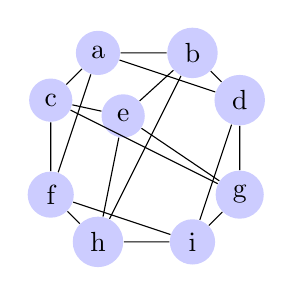
\begin{tikzpicture}
  [scale=.8,auto=left,every node/.style={circle,fill=blue!20},baseline]
  \node (n1) at (-0.75,1.5)      {a};
  \node (n2) at (0.75,1.5)    {b};
  \node (n3) at (-1.5,0.75)     {c};
  \node (n4) at (1.5,0.75)   {d};
  \node (n5) at (-0.35,0.5)   {e};
  \node (n6) at (-1.5,-0.75)    {f};
  \node (n7) at (1.5,-0.75)    {g};
  \node (n8) at (-0.75,-1.5)    {h};
  \node (n9) at (0.75,-1.5)    {i};
  
  \foreach \from/\to in {n1/n2,n1/n3,n1/n4,n1/n6,n2/n4,n2/n5,n2/n8,n3/n5,n3/n6,n3/n7,n4/n7,n4/n9,n5/n7,n5/n8,n6/n8,n6/n9,n7/n9,n8/n9}
    \draw (\from) -- (\to);
\end{tikzpicture} Observe the subgraph obtained by contracting the vertices a,d,f,i is the following graph: 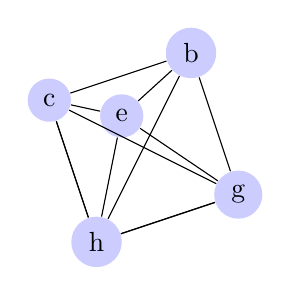
\begin{tikzpicture}
  [scale=.8,auto=left,every node/.style={circle,fill=blue!20},baseline]
  \node (n1) at (0.75,1.5)      {b};
  \node (n4) at (1.5,-0.75)   {g};
  \node (n5) at (-0.35,0.5)   {e};
  \node (n6) at (-1.5,0.75)    {c};
  \node (n9) at (-0.75,-1.5)    {h};
  
  \foreach \from/\to in {n1/n4,n1/n6,n4/n9,n6/n9,n1/n5,n1/n9,n4/n5,n4/n6,n4/n9,n5/n6,n6/n9,n5/n9}
    \draw (\from) -- (\to);
\end{tikzpicture} which is exactly $K_5$.
\\\\
\leavevmode\vadjust{\vspace{-\baselineskip}}\newline
    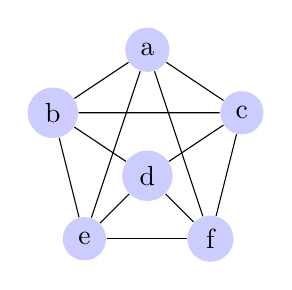
\begin{tikzpicture}
  [scale=.8,auto=left,every node/.style={circle,fill=blue!20},baseline]
  \node (n1) at (0,2)      {a};
  \node (n2) at (-1.5,1)    {b};
  \node (n3) at (1.5,1)     {c};
  \node (n4) at (0,0)   {d};
  \node (n5) at (-1,-1)   {e};
  \node (n6) at (1,-1)    {f};
  
  \foreach \from/\to in {n1/n2,n1/n3,n1/n5,n1/n6,n2/n3,n2/n4,n2/n5,n3/n4,n3/n6,n4/n5,n4/n6,n5/n6}
    \draw (\from) -- (\to);
\end{tikzpicture}
Is isomorphic to the planar graph: 
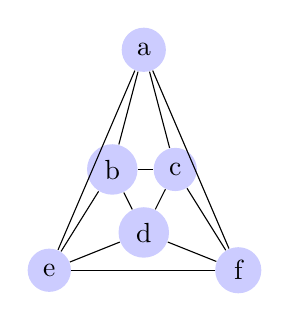
\begin{tikzpicture}
  [scale=.8,auto=left,every node/.style={circle,fill=blue!20},baseline]
  \node (n1) at (0,2)      {a};
  \node (n2) at (-0.5,0.1)    {b};
  \node (n3) at (0.5,0.1)     {c};
  \node (n4) at (0,-0.9)   {d};
  \node (n5) at (-1.5,-1.5)   {e};
  \node (n6) at (1.5,-1.5)    {f};
  
  \foreach \from/\to in {n1/n2,n1/n3,n1/n5,n1/n6,n2/n3,n2/n4,n2/n5,n3/n4,n3/n6,n4/n5,n4/n6,n5/n6}
    \draw (\from) -- (\to);
\end{tikzpicture}

\pagebreak
\item \begin{enumerate}
    \item By theorem 7.7.2, we know that $G$ is 2-colourable. Let $G$ be coloured by colours $A,B$, and let $e$ be any edge connecting an $A$-coloured vertex and a $B$-coloured vertex. We can do this without any loss of generality because $G$ is bipartite, and so every edge is an edge that connects an $A$-coloured vertex to a $B$-coloured vertex. Let us induct on the length of the path, $P$, we are replacing $e$ with in our subdivision. When the length of $P$ is 1, then clearly it is just $e$, and is 2-colourable, and hence 3-colourable. Then $P$ is 3-colourable for any length $\leq n$. Now take the length of $P=\{u_1,u_2,\ldots,u_{n+1}\}$ to be $n+1$. Since the endpoints of $P$ are two different colours, say $u_1$ is colour $A$ and $u_{n+1}$ is colour $B$. Then clearly the path $\{u_1,\ldots,u_n\}$ is a path of length $n$ and is $2-$colourable. Furthermore, we can colour $u_1$ colour $A$, then $u_2$ colour $C$, then $u_3$ colour $A$, etc. such that every colour will not be the colour of $u_{n+1}$. Then adding on $u_{n+1}$ to our path of 2 colours, $P$ is 3-colourable. Then by induction, $P$ is 3-colourable for any length. Then, for any size subdivision of any edge in $G$, that path is 3-colourable. Since all of the edges in $G$ connect vertices coloured $A$ to vertices coloured $B$ in $G$, then $H$ is 3-colourable. 
    
    \item Observe $K_{2,2}$: 
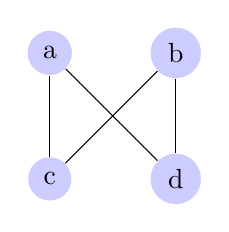
\begin{tikzpicture}
  [scale=.8,auto=left,every node/.style={circle,fill=blue!20},baseline]
  \node (n1) at (-1,1)      {a};
  \node (n2) at (1,1)    {b};
  \node (n3) at (-1,-1)     {c};
  \node (n4) at (1,-1)   {d};
  
  \foreach \from/\to in {n1/n3,n1/n4,n2/n3,n2/n4}
    \draw (\from) -- (\to);
\end{tikzpicture} and a subdivision of $K_{2,2}$, $H$: 
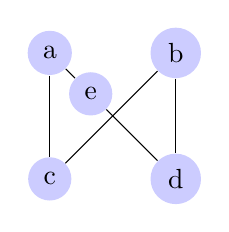
\begin{tikzpicture}
  [scale=.8,auto=left,every node/.style={circle,fill=blue!20},baseline]
  \node (n1) at (-1,1)      {a};
  \node (n2) at (1,1)    {b};
  \node (n3) at (-1,-1)     {c};
  \node (n4) at (1,-1)   {d};
  \node (n5) at (-0.35,0.35) {e};
  
  \foreach \from/\to in {n1/n3,n1/n5,n2/n3,n2/n4,n5/n4}
    \draw (\from) -- (\to);
\end{tikzpicture} Note that $K_{2,2}$ is 2-colourable since it is bipartite. It is also the 4-cycle. $H$, a subdivision of $K_{2,2}$, is the 5-cycle, and hence not bipartite, and not 2-colourable. 

\end{enumerate}
\pagebreak
\item \begin{enumerate}
    \item For $K_7:$ 
    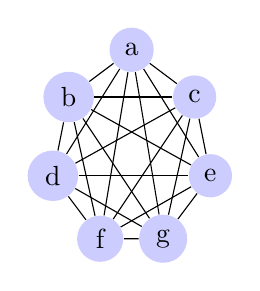
\begin{tikzpicture}
  [scale=.8,auto=left,every node/.style={circle,fill=blue!20},baseline]
  \node (n1) at (0,1.25)      {a};
  \node (n2) at (-1,0.5)    {b};
  \node (n3) at (1,0.5)     {c};
  \node (n4) at (-1.25,-0.75)   {d};
  \node (n5) at (1.25,-0.75)   {e};
  \node (n6) at (-0.5,-1.75)    {f};
  \node (n7) at (0.5,-1.75)     {g};
  
  \foreach \from/\to in {n1/n2,n1/n3,n1/n4,n1/n5,n1/n6,n1/n7,n2/n3,n2/n4,n2/n5,n2/n6,n2/n7,n3/n4,n3/n5,n3/n6,n3/n7,n4/n5,n4/n6,n4/n7,n5/n6,n5/n7,n6/n7}
    \draw (\from) -- (\to);
\end{tikzpicture} observe the complementary pair \\ 

$G:$     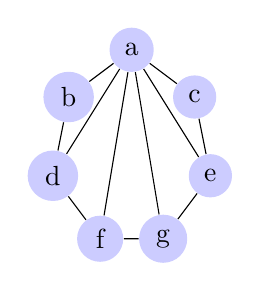
\begin{tikzpicture}
  [scale=.8,auto=left,every node/.style={circle,fill=blue!20},baseline]
  \node (n1) at (0,1.25)      {a};
  \node (n2) at (-1,0.5)    {b};
  \node (n3) at (1,0.5)     {c};
  \node (n4) at (-1.25,-0.75)   {d};
  \node (n5) at (1.25,-0.75)   {e};
  \node (n6) at (-0.5,-1.75)    {f};
  \node (n7) at (0.5,-1.75)     {g};
  
    \draw (n1) -- (n2);
    \draw (n1) -- (n3);
    \draw (n1) -- (n4);
    \draw (n1) -- (n5);
    \draw (n1) -- (n6);
    \draw (n1) -- (n7);
    \draw (n2) -- (n4);
    \draw (n3) -- (n5);
    \draw (n4) -- (n6);
    \draw (n5) -- (n7);
    \draw (n6) -- (n7);
  %  \draw (n6) -- (n2);
 %   \draw (n6) -- (n3);
%    \draw (n6) -- (n5);
    
\end{tikzpicture} $\quad\quad H:$    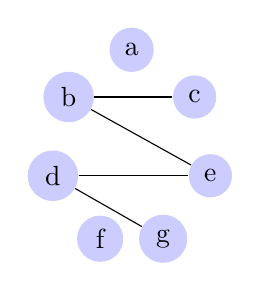
\begin{tikzpicture}
  [scale=.8,auto=left,every node/.style={circle,fill=blue!20},baseline]
  \node (n1) at (0,1.25)      {a};
  \node (n2) at (-1,0.5)    {b};
  \node (n3) at (1,0.5)     {c};
  \node (n4) at (-1.25,-0.75)   {d};
  \node (n5) at (1.25,-0.75)   {e};
  \node (n6) at (-0.5,-1.75)    {f};
  \node (n7) at (0.5,-1.75)     {g};

  
  \draw (n2) to (n3);
  \draw (n2) to (n5);
% \draw (n2) to (n7);
% \draw (n3) to (n4);
% \draw (n3) to (n7);
  \draw (n4) to (n5);
 \draw (n4) to (n7);
\end{tikzpicture} 



    \item Observe that for two subgraphs of $K_{11}$ to be planar, then both $|E(G)|\leq 3|V(G)|-6$, $|E(H)|\leq 3|V(H)|-6$ need to be satisfied. We know $|V(K_{11})|=11$, and so $|E(G)|$ can be at most $3*11-6=27$. Then since $H$ is the complement, and $|E(K_{11})|=55$, $H$ must have $55-27=28$ edges. But then $|E(H)|=28\geq 27 =3|V(K_{11})|-6$, hence $H$ cannot be planar if $G$ is planar. Clearly if the vertex set of $G$ or $H$ is not the vertex set of $K_{11}$, then this is even more true. Similarly, $G$ cannot be planar if $H$ is planar. 
\end{enumerate}

\pagebreak
\item \begin{enumerate}
    \item Since $G$ is planar, by Euler's formula we have $|V(G)|-|E(G)|+|f(G)|=1+c$, where $c$ is the number of components of $G$. If $G$ has no cycles, then we know $|V(G)|=|E(G)|+c$, where $c$ is the number of components. Plugging these formulas into each other, we get $|V(G)|=3|V(G)|-6+c\Rightarrow c=6-2|V(G)|$. Since $|V(G)|\geq4$, we get $c\leq -2$, which is clearly not true, so $G$ has a cycle. \\ 
    Since $G$ contains a cycle, by lemma 7.5.1, every face boundary contains a cycle. Then since a cycle has to have length at least three, every face has degree at least three, and so by handshaking lemma for faces, we have $3|f(G)|\geq 2|E(G)|=2(3|V(G)|-6)\Rightarrow |f(G)|\geq 2|V(G)|-4$. Then, plugging into Euler's formula, we have $|V(G)|-(3|V(G)|-6)+2|V(G)|-4\geq 1+c$. Since the $|V(G)|$'s cancel out, we are left with $1\geq c$. Since $c$ is a non-negative integer, and we know we have at least $4$ vertices, and hence $3*4-6$ edges, $c$ can not be the empty graph, and hence $c=1$, and therefore $G$ is connected. 
    
    
    \item By handshaking lemma for faces, we have $\sum_{F\in f(G)}d^*(F)=2|E(G)|$. But we know $|E(G)|=3|V(G)|-6$, so $\sum_{F\in f(G)}d^*(F)=6|V(G)|-12\Rightarrow |V(G)|=\frac{\sum_{F\in f(G)}d^*(F)+12}{6}$. Then plugging into Euler's formula and the equation given in the question, we get 
    \begin{align*}
    \frac{\sum_{F\in f(G)}d^*(F)+12}{6}-\left(3|V(G)|-6\right)+|f(G)|&=2 \\ 
    \frac{\sum_{F\in f(G)}d^*(F)+12}{6}-\left(3\frac{\sum_{F\in f(G)}d^*(F)+12}{6}-6\right)+|f(G)|&=2 \\ 
    \frac{\sum_{F\in f(G)}d^*(F)}{6}+2-\frac{\sum_{F\in f(G)}d^*(F)}{2}-6+6+|f(G)|&=2 \\
    \frac{\sum_{F\in f(G)}d^*(F)}{2}-\frac{\sum_{F\in f(G)}d^*(F)}{6}&=f|(G)|\\
    \sum_{F\in f(G)}d^*(F)&=3|f(G)|\\
    \end{align*}
    Note that a face cannot have degree 2 or less, (or else it would not be a face in our graph with a cycle, and $|V(G)|\geq4$), so every face has degree exactly 3.
\end{enumerate}

\pagebreak
\item Note that for $a\geq3$, and $b+c\geq3$, we can contract the vertices in one of $b$ or $c$ to create a complete bipartite graph, with the size of both partitions being greater than or equal to three, and hence it contains $K_{3,3}$ as a subdivision, and is not planar. Hence, $K_{a,b,c}$ is planar only when $a\leq2$ and $b+c\geq3$ are true, and $a\geq3$ and $b+c\leq2$ are true. For $a\geq3, b+c\leq2$, the triples $(a,b,c)$ such that these are true are just $(n,1,1)$, where $n\in\mathbb{N}$. For $a\leq2,b+c\geq3$, we first notice that if $b+c\geq5$, they are at least 2 and 3, in which case we have a subdivion of $K_{3,3}$, or they are at least 1 and 4, in which case we have a subdivision of $K_{5}$ if $a=2$ or one of $b,c>1$, and if $a=1$ and one of $b,c=1$, we get a case covered by the above triple. Then we need $3\leq b+c\leq4$. Then we get the triples $(1,2,1),(1,2,2),(2,2,1),(2,2,2)$, and removing repeated cases we get the triples $(2,2,2),(2,2,1)$. Then, all triples $(a,b,c)$ such that $K_{a,b,c}$ is planar are: $(a,1,1), (2,2,2), (2,2,1)$.

\end{enumerate}

\end{document}
